\documentclass[a4paper,class=article,border=10pt,tikz]{standalone}

%mypackages
\usepackage{pythontex}
\usepackage{pgfplots}
\usepackage{amsmath}
\usepackage{titlesec}
\usepackage{tikz}
\usetikzlibrary{shapes.geometric}
\usetikzlibrary{positioning}
\usetikzlibrary{snakes,calc,positioning,patterns,angles,quotes,decorations.pathmorphing,decorations.markings}
% \titleformat{<command>}[<shape>]{<format>}{<label>}{<sep>}{<before-code>}[<after-code>]
%\titleformat{\section}{\normalfont\Large\bfseries}{\thesection.}{10pt}{}
% \titlespacing{<command>}{<left>}{<before-sep>}{<after-sep>}
%\titlespacing{\section}{0pt}{14pt}{7pt}

%\titleformat{\subsection}{\normalfont\itshape}{\thesubsection.}{10pt}{}
%\titlespacing{\subsection}{0pt}{12pt}{6pt}
% set font encoding for PDFLaTeX, XeLaTeX, or LuaTeX
\usepackage{ifxetex,ifluatex}
\if\ifxetex T\else\ifluatex T\else F\fi\fi T%
  \usepackage{fontspec}
\else
  \usepackage[T1]{fontenc}
  \usepackage[utf8]{inputenc}
  \usepackage{lmodern}
\fi

\usepackage{hyperref}


\title{Title of Document}
\author{Name of Author}

% Enable SageTeX to run SageMath code right inside this LaTeX file.
% http://doc.sagemath.org/html/en/tutorial/sagetex.html
% \usepackage{sagetex}

% Enable PythonTeX to run Python – https://ctan.org/pkg/pythontex
% \usepackage{pythontex}

\begin{document}

 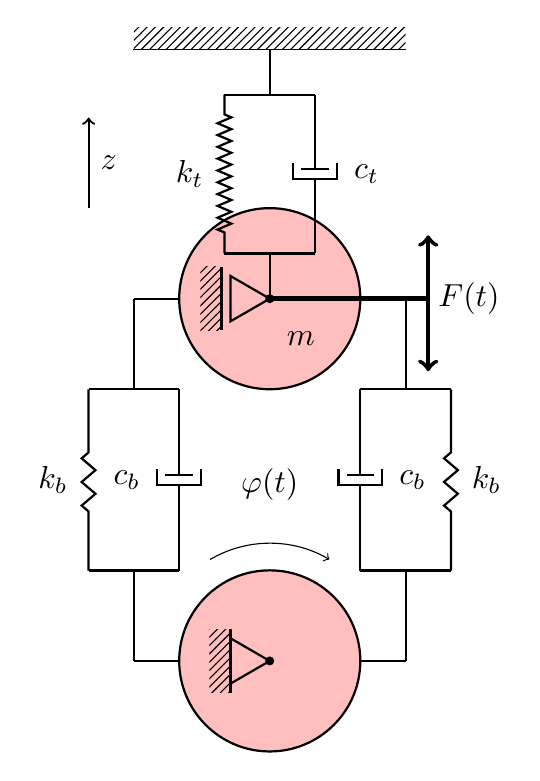
\begin{tikzpicture}[scale=1.15, transform shape]
 
\tikzstyle{spring}=[thick,decorate,decoration={zigzag,pre length=0.75cm,post length=0.75cm,segment length=0.3cm}]
\tikzstyle{tspring}=[thick,decorate,decoration={zigzag,pre length=0.25cm,post length=0.25cm,segment length=0.15cm}]
\tikzstyle{damper}=[thick,decoration={markings,  
  mark connection node=dmp,
  mark=at position 0.5 with 
  {
    \node (dmp) [thick,inner sep=0pt,transform shape,rotate=-90,minimum width=15pt,minimum height=3pt,draw=none] {};
    \draw [thick] ($(dmp.north east)+(2pt,0)$) -- (dmp.south east) -- (dmp.south west) -- ($(dmp.north west)+(2pt,0)$);
    \draw [thick] ($(dmp.north)+(0,-5pt)$) -- ($(dmp.north)+(0,5pt)$);
  }
}, decorate]
\tikzstyle{ground}=[fill,pattern=north east lines,draw=none,minimum width=0.75cm,minimum height=0.4cm]
\tikzstyle{damper}=[thick,decoration={markings,  
  mark connection node=dmp,
  mark=at position 0.5 with 
  {
    \node (dmp) [thick,inner sep=0pt,transform shape,rotate=-90,minimum width=15pt,minimum height=3pt,draw=none] {};
    \draw [thick] ($(dmp.north east)+(2pt,0)$) -- (dmp.south east) -- (dmp.south west) -- ($(dmp.north west)+(2pt,0)$);
    \draw [thick] ($(dmp.north)+(0,-5pt)$) -- ($(dmp.north)+(0,5pt)$);
  }
}, decorate]

\node (crank) [draw,fill=pink,circle,outer sep=0pt, thick,minimum size=2cm] at (0cm,-4cm) {};
\node (blower) [label={[label distance=-0.75cm]-75:$m$},draw,fill=pink,circle,outer sep=0pt, thick,minimum size=2cm] at (0,0cm) {};
\node (ground) [ground,anchor=north,minimum width=3cm,minimum height=0.2cm] at (0,3cm) {};


\draw [thick,rotate=-90] (crank.center)--++ (-60:0.5)--++(-0.5,0) node[midway] (support_end){}--++ (60:0.5);
\fill [black] (crank.center) circle (0.05);
\node (fixed_support) [anchor=north,ground,outer sep=0pt,thick,yshift=0cm,minimum height=0.1cm ,minimum width=0.7cm,rotate=-90]  at (support_end) {};

\draw [thick] (fixed_support.north west) -- (fixed_support.north east);
% 
\draw [thick,rotate=-90] ([yshift=-0cm]blower.center) --++ (-60:0.5) --++(-0.5,0)  node (support_start)[midway] {}  --++ (60:0.5);
% 
\node (floating_support) [ground,outer sep=0pt,thick,anchor=north,minimum height=0.05cm ,minimum width=0.7cm,rotate=-90,yshift=-0.1cm]  at (support_start) {};
% 
\draw [thick] (floating_support.north west) -- (floating_support.north east);
\fill [black] (blower.center) circle (0.05);


\draw (ground.south west) -- (ground.south east);

\draw[thick] (crank.180) --++ (-0.5cm,0) node (cl) {};
\draw[thick] (crank.0) --++ (0.5cm,0) node (cr) {};
\draw[thick] (blower.180) --++ (-0.5cm,0) node (bl) {};
\draw[thick] (blower.0) --++ (0.5cm,0) node (br) {};

\draw[thick] (bl.center)--++(0,-1cm) node (b2l) {};
\draw[thick] (br.center)--++(0,-1cm) node (b2r) {};
\draw[thick] (cl.center)--++(0,1cm) node (c2l) {};
\draw[thick] (cr.center)--++(0,1cm) node (c2r) {};

\draw[thick] (c2l.center)--++(-0.5cm,0) node (cll) {};
\draw[thick] (c2l.center)--++(0.5cm,0) node (clr) {};
\draw[thick] (c2r.center)--++(-0.5cm,0) node (crl) {};
\draw[thick] (c2r.center)--++(0.5cm,0) node (crr) {};
\draw[thick] (b2l.center)--++(0.5cm,0) node (blr) {};
\draw[thick] (b2l.center)--++(-0.5cm,0) node (bll) {};
\draw[thick] (b2r.center)--++(0.5cm,0) node (brr) {};
\draw[thick] (b2r.center)--++(-0.5cm,0) node (brl) {};

\draw [spring]  (cll.center) -- (bll.center) node (k_b1) [left,midway,xshift=-0.1cm] {$k_b$};
\draw [spring]  (crr.center) -- (brr.center) node (k_b2) [right,midway,xshift=0.1cm] {$k_b$};

\draw [damper]  (clr.center) -- (blr.center) node (k_b1) [left,midway,xshift=-0.3cm] {$c_b$};
\draw [damper]  (crl.center) -- (brl.center) node (k_b2) [right,midway,xshift=0.3cm] {$c_b$};

\draw[thick] (ground.270)--++(0,-0.5cm) node (g2n) {};
\draw[thick] (g2n.center)--++(-0.5cm,0) node (n2s) {};
\draw[thick] (g2n.center)--++(0.5cm,0) node (n2d) {};
\draw[thick] (blower.center)--++(0,0.5cm) node (b2n) {};
\draw[thick] (b2n.center)--++(-0.5cm,0) node (n2ss) {};
\draw[thick] (b2n.center)--++(0.5cm,0) node (n2dd) {};

\draw [tspring]  (n2s.center) -- (n2ss.center) node (k_t) [left,midway,yshift=0cm,xshift=-0.1cm] {$k_t$};
\draw [damper]   (n2dd.center) -- (n2d.center) node (c_t) [right,midway,yshift=0cm,xshift=0.3cm] {$c_t$};

\coordinate (end2) at (-2.5,0.25) ;

\coordinate (end1) at (2.5,0.25) ;

\draw [-latex,ultra thick,<->,rotate=90] (blower.center) ++ (-0.8cm,-1.75cm) -- +(1.5cm,0cm);
\draw[ultra thick] (blower.center)--++(1.75cm,0);
\node (ft) at (2.2cm,0) {$F(t)$};
 \pic [draw, <-, "$ \varphi(t) $", angle eccentricity=1.5, angle radius=1.3cm] {angle = end1--crank--end2};
\draw[thick,->] (-2,1) -- (-2,2) node[midway, right] {$z$};



\end{tikzpicture}
\end{document}